\section{Tidsforlængelse} \label{sec:Tidsforlaengelse}
En spøjs konsekvens af relativitetsteorien er, at tidens gang afhænger af, hvor hurtigt man bevæger sig. For at kunne snakke om tid bliver vi først nødt til at have et ur, men vi kan ikke bare gøre brug af et hvilket som helst ur. Vi har brug for et ur, der eksplicit udnytter lysets hastighed. Vi vil derfor se på det såkaldte lysur. Lysuret består af to perfekte spejle overfor hinanden, og mellem disse er en lyspuls, der bevæger sig frem og tilbage spejlene, se figur \ref{fig:Lysur}a. At det på ingen måde er praktisk at fremstille et sådant ur er ikke et problem, vi vil blot regne på det.

\begin{figure}
    \centering
    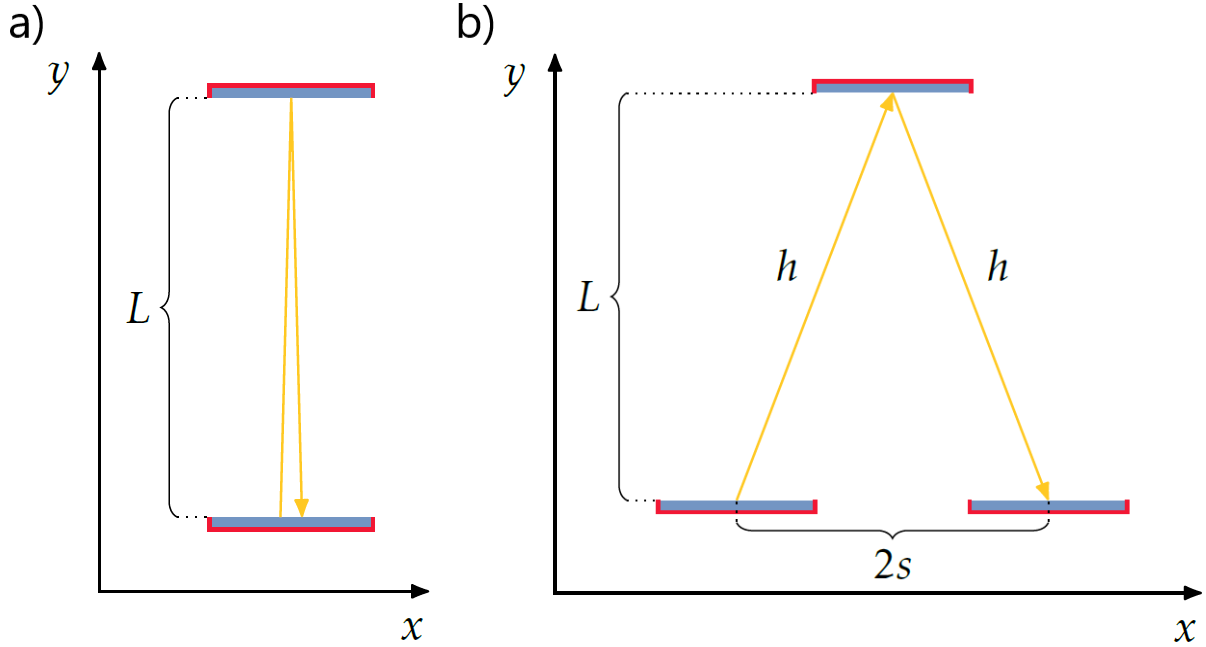
\includegraphics[width=.8\textwidth]{SR/billeder/Lysur.png}
    \caption{Lysuret. a) Stillestående (eller blot set fra hvilesystemet). Lysstrålen bevæger sig præcis lodret men er her blot tegnet en smule forskudt, så pricippet i lysuret kan ses. b) Bevægende med konstant hastighed $v$. Kilde: figur 2.1 og 2.2 i \cite{uggerhojSpecielRelativitetsteori2016}.}
    \label{fig:Lysur}
\end{figure}

Lyset vil bevæge sig mellem de to spejle med lysets hastighed. Tiden, som det vil tage lyset at tilbagelægge en afstand $L$ mellem de to spejle, vil derved være $L/c$. Det betyder, at urets periode, som er tiden det tager lyset at nå frem og tilbage igen mellem spejlene, når uret er i hvile -- i et hvilesystem -- vil være
\begin{equation} \label{rel:hvile}
T_0=\frac{2L}{c} \: .
\end{equation}
Uret sættes nu i bevægelse med konstant hastighed $v$ vinkelret på lysstrålen i uret.
Lad os kalde den afstand, som uret rejser i løbet af en halv periode, for $s$. Da er
\begin{equation} \label{rel:halv_periode}
s=\frac{vT}{2} \: .
\end{equation}
Hvis man observerer lyset fra lysurets hvilesystem -- systemet, som bevæger sig med konstant hastighed $v$ i samme retning som lysuret -- så vil lyset se ud til stadig at bevæge sig lodret op og ned. Lyset skal ramme samme punkt på spejlet uanset om lysuret betragtes i et inertialsystem i hvile eller i bevægelse. Tilsvarende skal lyset bevæge sig i en ret linje, i det system hvor lysuret bevæger sig, da lysets bane er en ret linje i det system, hvor uret er i hvile. Hvis ikke det var tilfældet, så ville naturens love være forskellige i de to inertialsystemet, hvilket således ville bryde med relativitetsprincippet. Observerer man nu lyset fra et system, hvor lysuret bevæger sig med den konstante hastighed $v$ vinkelret på lysets bevægelse, så må lyset i dette system have en `skrå' bevægelse -- bevæge sig i en skrå bane, som siderne på en ligevinklet trekant -- da lyset må følge resten af uret, se figur \ref{fig:Lysur}b. Lysets hastighed, $c$, skal dog være uændret ifølge det andet postulat.
Lad os kalde den `skrå' afstand, som lyset bevæger sig, for $h$.
Vi kan nu benytte Pythaoras sætning til af sammenkæde $h$, $s$ og $L$:
\begin{equation}
h^2=L^2+s^2 \: .\label{rel:pyt}
\end{equation}
Afstanden $h$ må blive tilbagelagt på en halv periode, da det tager en hel periode at nå fra det nederste spejl til det øverste og tilbage igen. Idet lysuret er i bevægelse betegner vi perioden med $T$, og den findes ved
\begin{equation}
T=\frac{2h}{c} \label{rel:per}\: .
\end{equation}
Vi kan isolere længderne $L$, $h$ og $s$ fra urets periode i de to systemer, ligning \eqref{rel:hvile}, \eqref{rel:halv_periode} og \eqref{rel:per} og indsætte disse i Pythagoras sætning, ligning \eqref{rel:pyt}, for at få:
\begin{equation}
\frac{T^2c^2}{4}=\frac{T_0^2c^2}{4}+\frac{T^2v^2}{4} \: .
\end{equation}
Her kan $T$ isoleres
\begin{equation} \label{rel:Tidsforlaengelse}
    T=\frac{T_0}{\sqrt{1-\frac{v^2}{c^2}}}=\gamma T_0 \: .
\end{equation}
Udtrykket $(1-v^2/c^2)^{-1/2}$ er så almindeligt i relativitetsteorien, at det har fået sit eget symbol, $\gamma$. Denne kaldes Lorentzfaktoren, men bliver også til kaldet gammafaktoren, grundet symbolet for denne ($\gamma$), og er givet ved:
\begin{equation}
    \gamma =\frac{1}{\sqrt{1-\frac{v^2}{c^2}}} \: .
\end{equation}
For en observatør, der rejser med lysuret, er uret oplagt i hvile, hvorfor den observerede periode for lysuret vil være $T_0$ i stedet for $T = \gamma T_0$. Så de to observatører ser uret gå forskelligt.
Hvordan kan vi få det til at give mening?
Det kan virke mystisk, men den lettest måde at få det til at give mening, er at tiden går langsommere, desto hurtigere uret bevæger sig.
Derudover er der intet, der adskiller lysuret fra andre måder at opleve tiden, ud over at det er let at regne på.

Man kunne spørge sig selv: Hvorfor $gamma$? Det kommer af, at der er to andre faktorer, der har fået $\alpha$ og $\beta$, så man har givet den tredje konstant det tredje græske bogstav.
Betafaktoren er forholdet imellem $v$ og lysets hastighed:
\begin{equation}
    \beta=\frac{v}{c} \: .
\end{equation}
Alfafaktoren er 1 over gammafaktoren, så da den ikke fortæller noget nyt bruges den ikke rigtigt:
\begin{equation}
    \alpha=\sqrt{1-\frac{v^2}{c^2}} \: .
\end{equation}

Det kan virke spøjst at tidens gang afhænger af hvor hurtigt man bevæger sig, men der er naturlige fænomener, der afhænger af tidsforlængelse.
Når solvinden rammer Jordens atmosfære i en højde af ca. \SI{10}{\kilo\metre}, dannes der myoner\footnote{Myonen er en tung variant af en elektron, for mere information om myonen, se kapitel \ref{chap:Partikelfysik} om partikelfysik.}
Myonerne dannes med en hastighed tæt på lysets hastighed.
Myoner er ustabile partikler, og de henfalder ret hurtigt.
De har en halveringstid i hvile på \SI{1,5}{\micro\second}.
Uden relativistiske effekter ville det betyde at
\begin{gather}
    L_\text{halv}=t_\text{halv}c=\SI{450}{\metre} \: ,
\end{gather}
hvor $L_\text{halv}$ er afstanden, som myonerne ville tilbagelægge, før halvdelen af dem er henfaldet. Efter \SI{10}{\kilo\metre} burde praktisk talt alle myonerne være henfaldet.
Dog når en stor del af myonerne Jordens overflade, hvilket kan forklares ved, at tidet for myonerne går langsommere, da de er i bevægelse, hvorfor de fra Jorden ser ud til at leve længere end deres hvilehalveringstid tillader.

Men hvad så med situationen set fra myonerne?
Myonerne er i hvile i forhold til dem selv, så her går tiden, som vi ville forvente.
Men med deres korte levetid kan myonerne ikke tilbagelægge de \SI{10}{\kilo\metre} ned til Jordens overflade.
Vi kan ikke have to modstridende resultater, da det strider imod både sund fornuft -- og ikke mindst -- imod relativitetsprincippet.
Det viser sig ikke at være et problem, da det ikke kun er tid, der afhænger af observatøren, men også afstande, hvilket vi vil se på i afsnit \ref{sec:Laengdeforkortelse}.

Tiden i hvilesystemet kaldes også for egentiden, $\tau$ (det græske bogstav \emph{tau}), og siden det er for et specifikt inertialsystem, kan alle observatører blive enige om egentiden. 